\begin{frame}{Experimental Results: RL Lab}
\begin{figure}
    \centering
    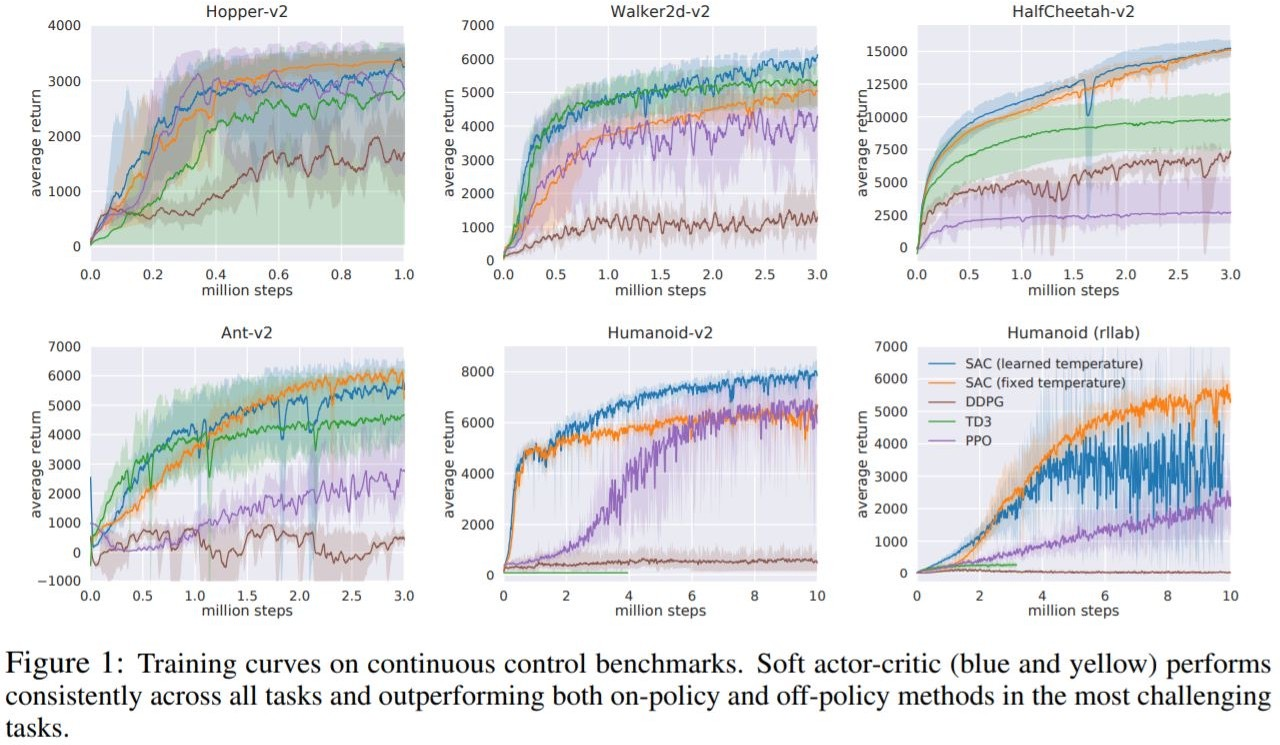
\includegraphics[width=\textwidth,height=0.78\textheight,keepaspectratio]{images/soft-actor-critic/figures/sac-rllab-grid.jpg}
    \caption*{\footnotesize Figure 1: Training curves on continuous control benchmarks. Soft actor-critic (blue and yellow) performs consistently across all tasks and outperforming both on-policy and off-policy methods in the most challenging tasks.}
\end{figure}
\begin{flushright}
    \tiny\url{https://arxiv.org/abs/1801.01290}
\end{flushright}
\end{frame}
\begin{frame}{Experimental Results: Robustness}
\begin{columns}[T]
\begin{column}{0.5\textwidth}
\small
\textbf{Task:} Sawyer arm trained with SAC to stack a block.
\vspace{0.4em}
\begin{itemize}
    \item Evaluated under \emph{perturbations unseen at training time} (a human pushes the block / arm)
    \item The stochastic, entropy-regularised policy adapts to off-distribution states
    \item A deterministic policy would freeze on the trained trajectory
\end{itemize}
\end{column}
\begin{column}{0.45\textwidth}
\centering
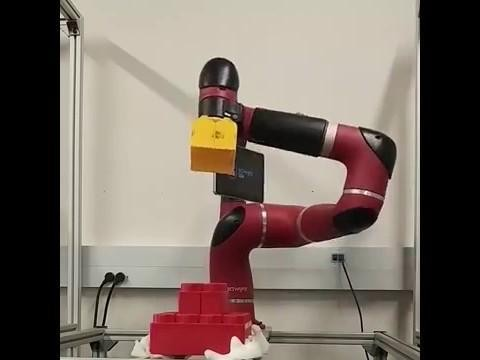
\includegraphics[width=\linewidth,height=0.75\textheight,keepaspectratio]{images/soft-actor-critic/figures/sac-robustness-robot.jpg}
\end{column}
\end{columns}
\begin{flushright}
    \tiny\url{https://sites.google.com/view/sac-and-applications}
\end{flushright}
\end{frame}
